%% paper.tex


%\documentclass[pldi]{sigplanconf-pldi16}
\documentclass[10pt]{sigplanconf}
% standard LaTeX packages

% standard LaTeX packages
%\usepackage{changebar}

\usepackage{balance}
\usepackage{alltt}
\usepackage{amsmath}
\usepackage{balance}
\usepackage{booktabs}
\usepackage{fixltx2e}
\usepackage{graphicx}
\usepackage{boxedminipage}
\usepackage{hyperref}
\usepackage{nicefrac}
\usepackage{subfig}
\usepackage{xcolor}
\usepackage{setspace}
\usepackage{xspace}
\usepackage{multirow}
\usepackage{colortbl}
\usepackage{amsfonts} 
\usepackage{blindtext}
\usepackage{chngpage}
\usepackage{listings}
\usepackage{mathtools}
\usepackage{amssymb}
\usepackage{pifont}
%\usepackage{pgfplotstable}

\usepackage[linesnumbered, vlined, ruled]{algorithm2e}
% font selection
%\usepackage{courier}
%\usepackage[scaled]{helvet}
\usepackage{mathptmx}
\usepackage{times}

% custom packages for this paper
\usepackage{double-blind}
\usepackage{shared-affiliation}

\usepackage[numbers,sort&compress,square]{natbib}

\lstset{
  basicstyle=\tiny,
  columns=fullflexible,
  numbersep=5pt,
  numberstyle=\scriptsize,
  showstringspaces=false,
  escapeinside={/*@}{@*/},
  belowcaptionskip=1\baselineskip,
  language=C,
  showstringspaces=true,
  keywordstyle=\bfseries,
  commentstyle=\itshape,
}


%\pgfplotstableset{
%    color cells/.style={
%        col sep=comma,
%        string type,
%        postproc cell content/.code={%
%                \pgfkeysalso{@cell content=\rule{0cm}{2.4ex}\cellcolor{black!##10}\pgfmathtruncatemacro\number{##1}\ifnum\number>5\color{white}\fi##1}%
%                },
%        columns/x/.style={
%            column name={},
%            postproc cell content/.code={}
%        }
%    }
%}


\makeatletter
\def\@copyrightspace{\relax}
\makeatother

\captionsetup{format=default, font=bf}


\newcommand*{\Scale}[2][4]{\scalebox{#1}{$#2$}}%
\newcommand{\comment}[1]{{}}

%% taken from unknown.sty
%\DeclareCaptionType{copyrightbox}

\sloppy

\begin{document}

\title{
  Learning from Big Security
}

\input macros.tex

%\numberofauthors{2}
\authorinfo{Linhai Song}
           {University of Wisconsin--Madison}
           {\{songlh\}@cs.wisc.edu}
\maketitle
\begin{abstract}
\input section/abstract.tex
\end{abstract}


\section{Introduction}

As a free online service, VirusTotal~\cite{virustotal} analyzes files submitted by real-world users to identify many different kinds of malwares, 
like viruses, worms, trojans, and so on. 
VirusTotal applies different antivirus engines to each submitted file and generate an aggregated reports. 
All submitted files and generated reports are saved and can be accessed through public API. 

The repository on VirusTotal provides a good source to conduct data mining. 
Firstly, there are huge amount of data on VirusTotal.
Figure~\ref{fig:subnum} shows that there were more than 40 million suspicious files 
submitted last November. 
This amount of data makes VirusTotal a rough estimation of malwares in the real world. 
Secondly, all data on VirusTotal are labeled by state-of-the-art antivirus techniques. 
VirusTotal updates each antivirus engine every 5 minutes. 
Besides whether a given a submitted file is detected by an antivirus engine, VirusTotal also keeps exact detection tag returned by each engine. 
There are also online active malware researchers, 
who can comment and vote each submitted file and serve as an important supplement of antivirus engines. 
We believe mining data on VirusTotal could enable many ``Big Security'' applications. 

In industry, antivirus vendors widely use VirusTotal to identify false negatives and false positives of their products. 
They only utilize VirusTotal reports separately for each single suspicious file, but fail to leverage the whole repository. 
In academia, researchers began to pay attention to correlations among different VirusTotal reports. 
For example, {\bf [ToDo: discuss Heqing's work]}
We believe there are much more research opportunities through mining VirusTotal. 

In this paper, we view data on VirusTotal as a stream, based on each file’s submission time, and design two stream mining applications: 
\textit{hot malware family mining} and \textit{malware prediction}. 
There are possibly infinite malware families. 
Hot malware family mining can precisely identify malware families, 
which occupy more than a given percentage of total malwares, by using a constant number of counters.
Malwares does not appear uniformly across different malware families or across time, 
and they appear in bursts. 
We built a cache-based algorithm to predict malwares in which families would appear in the near future. 

\begin{figure}[t!]
\begin{center}
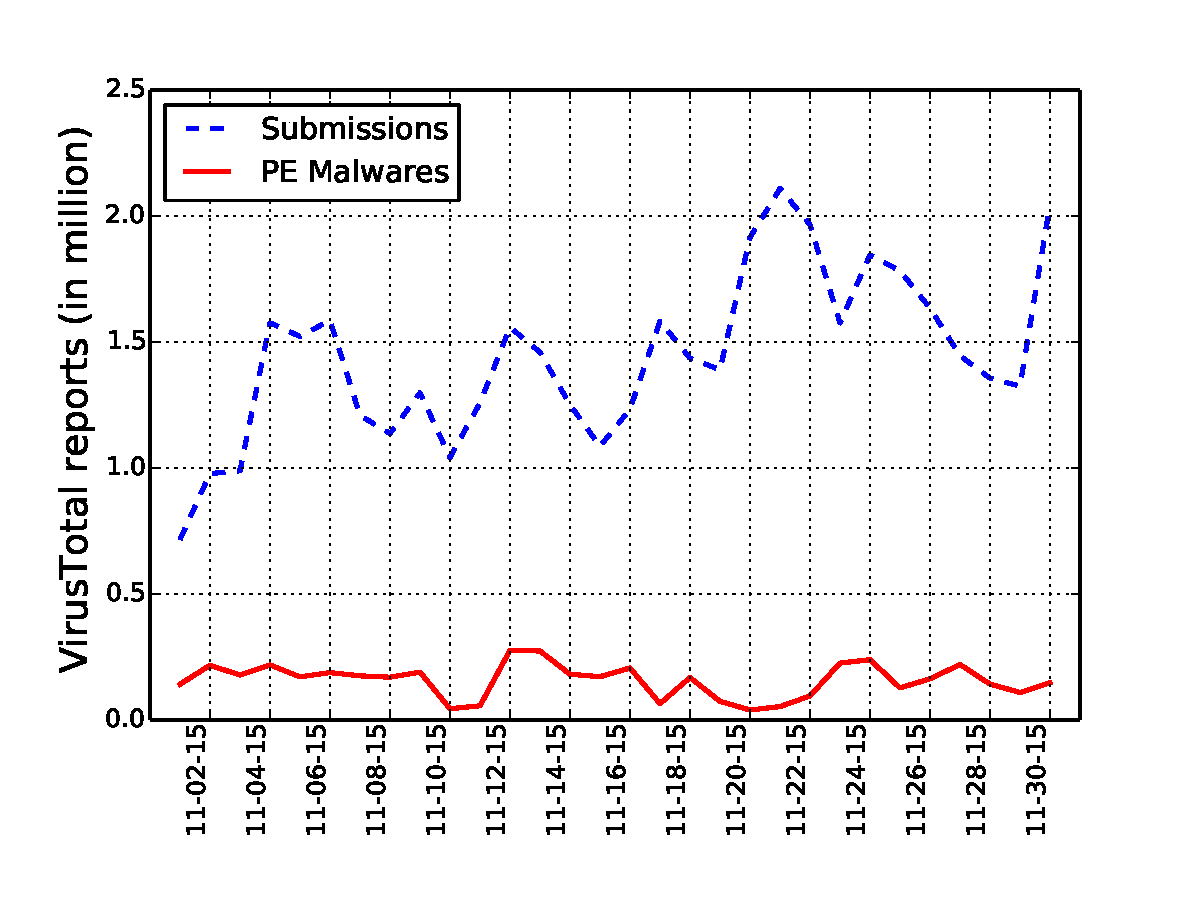
\includegraphics[width=3.0in]{figure/nov}
\caption{The number of files submitted to VirusTotal last November. }
\label{fig:subnum}
\end{center}
\end{figure}

In summary, we made the following contributions in this paper:

\begin{itemize}

\item We collect data submitted to VirusTotal last November, 
and briefly analyze these data to understand the characteristics of VirusTotal repository (Section~\ref{sec:meth}). 
\item We build two stream mining applications, one could identify hot malware family in a constant number of counters (Section~\ref{sec:hot}), 
and the other could predict malwares in the near future (Section~\ref{sec:predict}). 
Experimental results show that we can cover all hot malware family with a very few false positives, and we can predict future malwares with a high precision.
\item We discuss the future research opportunities through mining data on VirusTotal (Section~\ref{sec:oppo}), 
and demonstrate the feasibility by using our experience of building stream mining applications. 

\end{itemize}




%\input{related}
%\input{conclusion}

%%\balance
%\begin{spacing}{0.65}

\balance
{
\bibliographystyle{abbrvnat}
\bibliography{security} 
}
%\end{spacing}
\end{document}

% Local variables:
% TeX-PDF-mode: t
% TeX-master: t
% End:

% LocalWords:  Crug cci
